\appendix

\chapter{Appendix}
Appendix content goes here.

\section{Mockups}
After the second meeting with the customer, the group had a sketch that was to be used as a starting point for the mock-up application.
\pagebreak
\begin{figure}[here]
\setlength\fboxsep{0pt}
\setlength\fboxrule{1pt}
\fbox{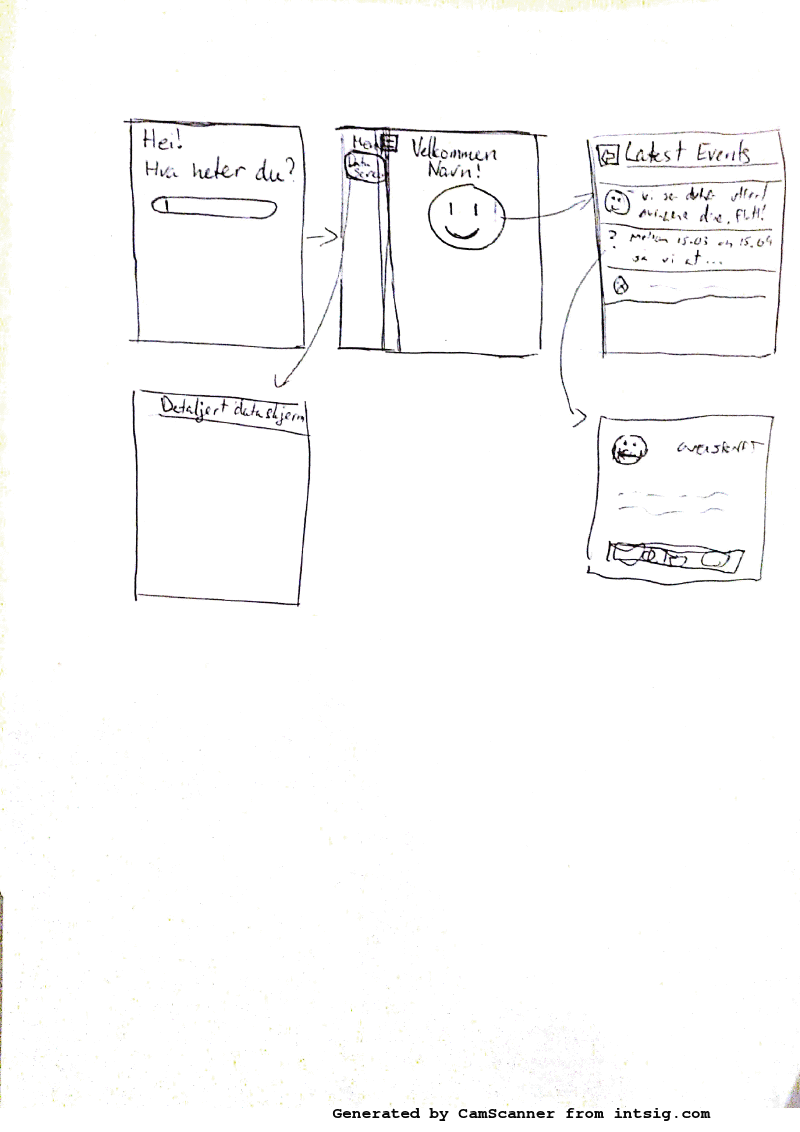
\includegraphics[trim = 20mm 180mm 0mm 20mm, clip, width=\linewidth]{Res/mockupV2}}
\caption{A mockup of the program flow, text is just scribbling}
\label{fig:mockupV2}
\end{figure}


\section{Reports}
The work done was described as short periods called sprints. 
\begin{figure}
\caption{Short summary of work done sorted by sprint}
\begin{tabular}{|c|c|p{7cm}|}
\hline
Sprint nr. & Date & Summary\\
\hline
Sprint 1: & 03.02.13 - 08.02.13 & Developing user stories and paper prototypes of the GUI.\\ 
\hline
Sprint 2: & 08.02.13 - 15.02.13 & Developing a mock-up application demonstrating the GUI.\\
\hline
Sprint 3: & 15.02.13 - 22.02.13 & Improving UI and functionality for the prototype, researching medicinal factors. \\
\hline
Sprint 4: & 22.02.13 - 01.03.13 & Improving secondary functionality for the prototype (settings, statistics, relatives screens),researching content-providers and alternative solutions. \\
\hline
Sprint 5: & 01.03.13 - 07.03.13 & Creating content-provider, creating presentation, finishing secondary screens (as described above), including pedometer, writing test-cases.\\
\hline
\end{tabular} 
\label{tab:sprintList}
\end{figure}
\newpage

\section{Meeting summaries}
Regular status reports was a part of necessary documentation. Of particular importance was reports to the supervisor, and reports done to the other group members. This status report was written during sprint 4. The reports were included in chronological order.


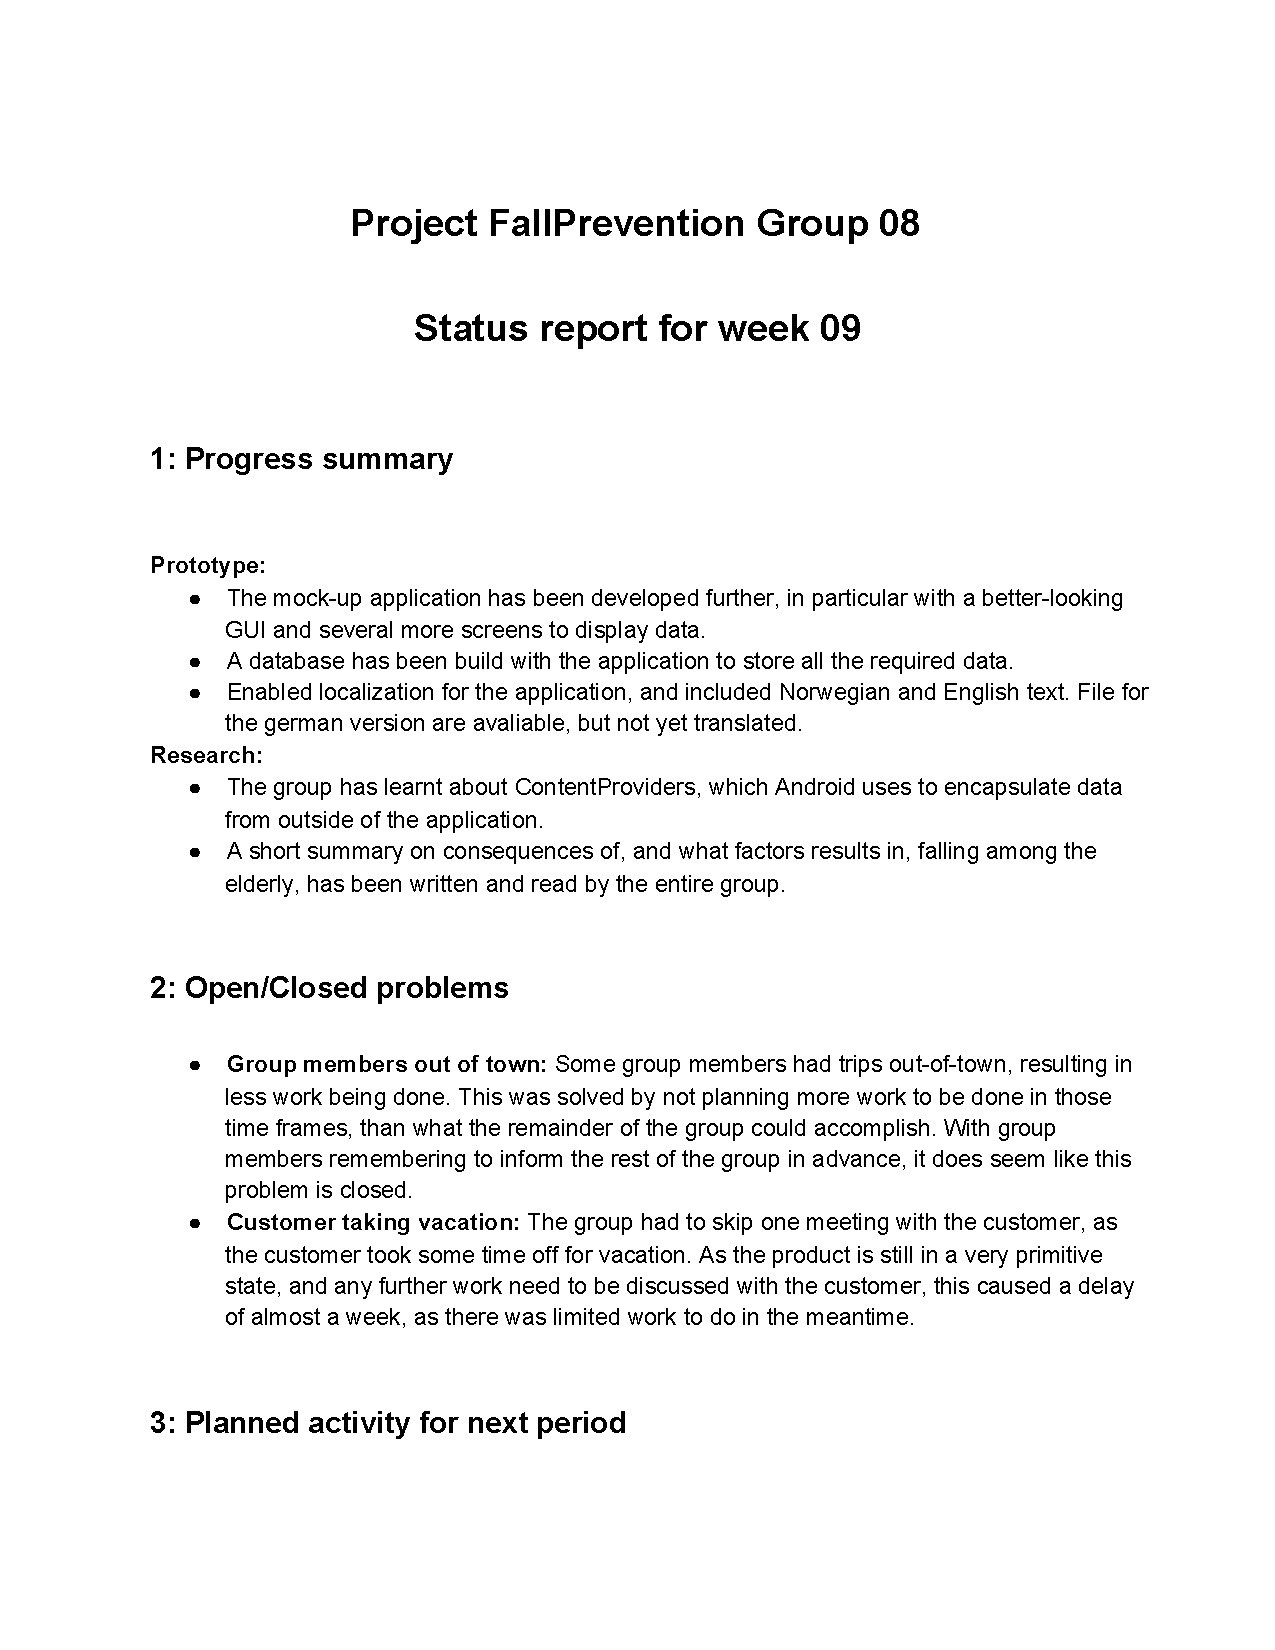
\includepdf[pages={-}]{Res/StatusReportWeek9}

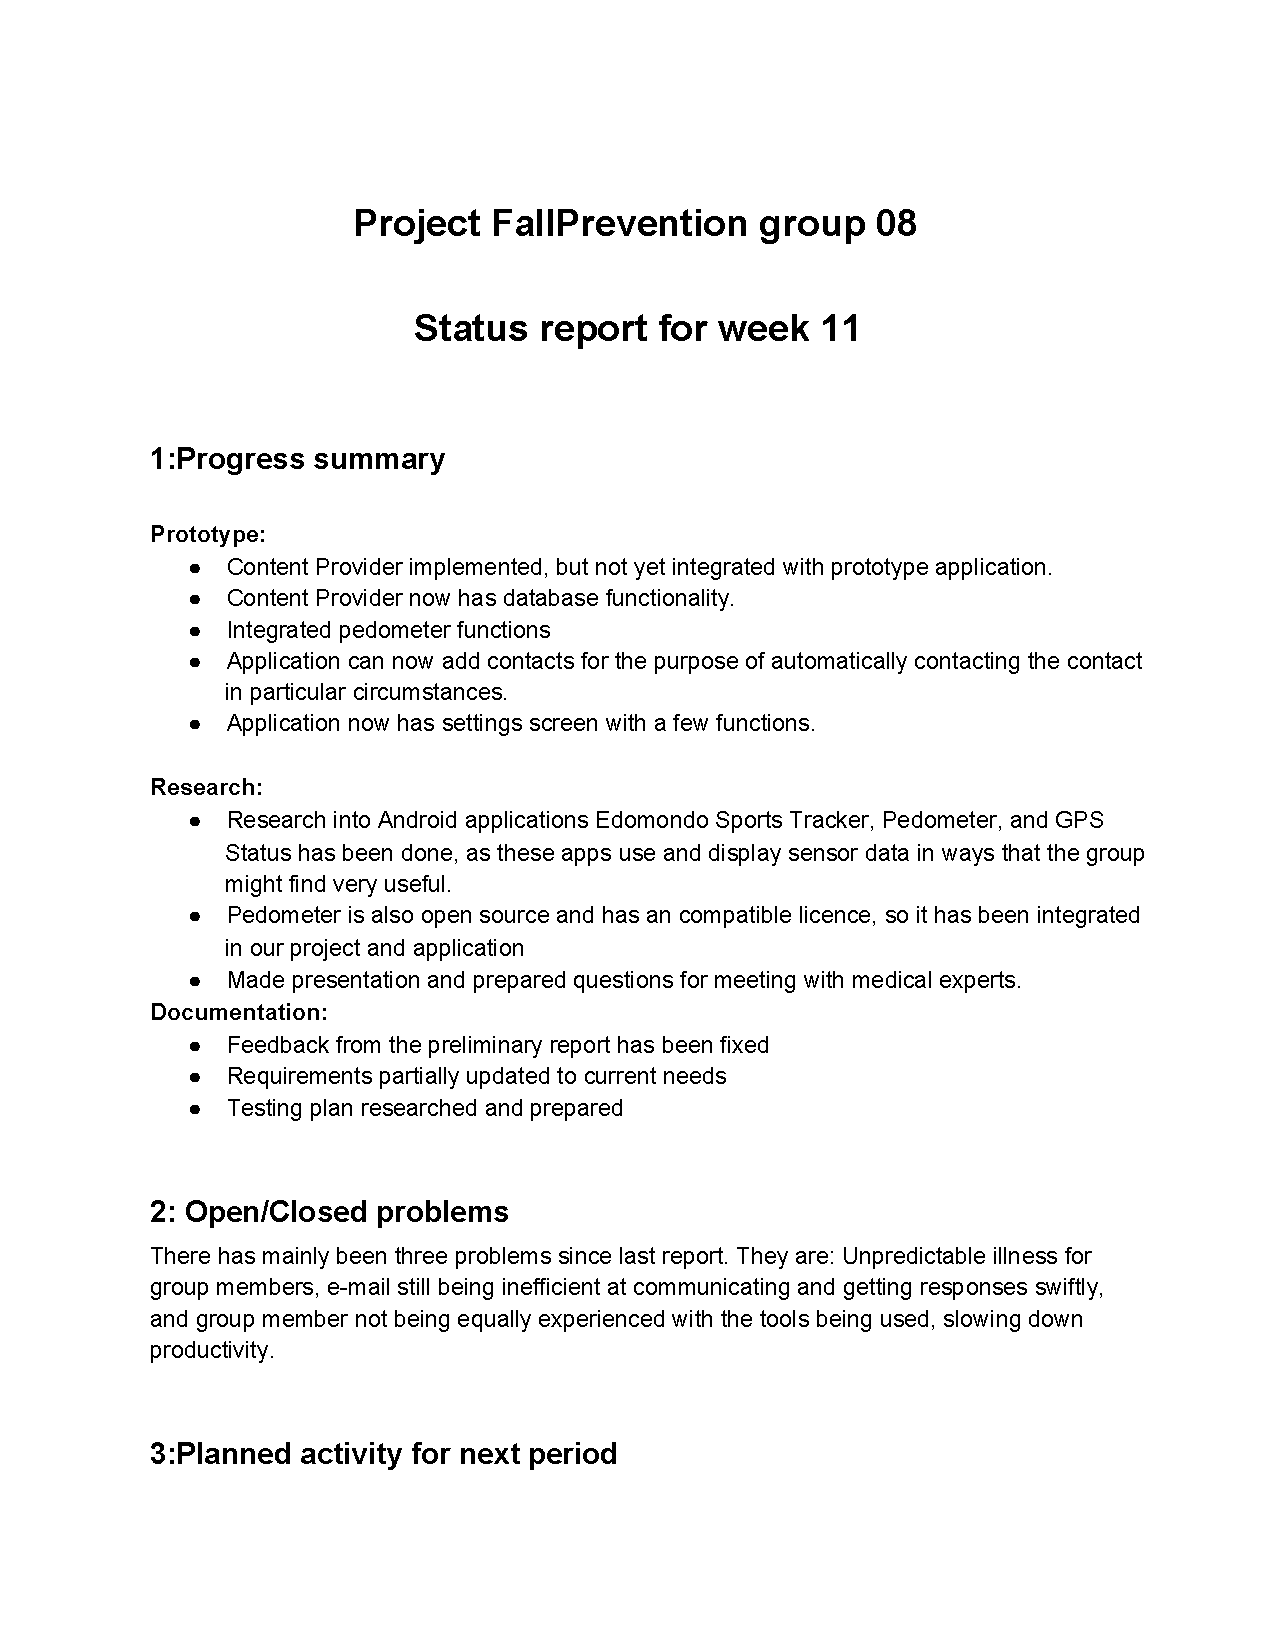
\includepdf[pages={-}]{Res/StatusReportWeek11}

\section{Alternate Solutions}
There was several other open source programs and commercial programs used to solve related problems. In some cases the team could import and make use of the open source programs, and in others the team could be inspired by design and well-made interfaces and functions. Here is the report, included as written:
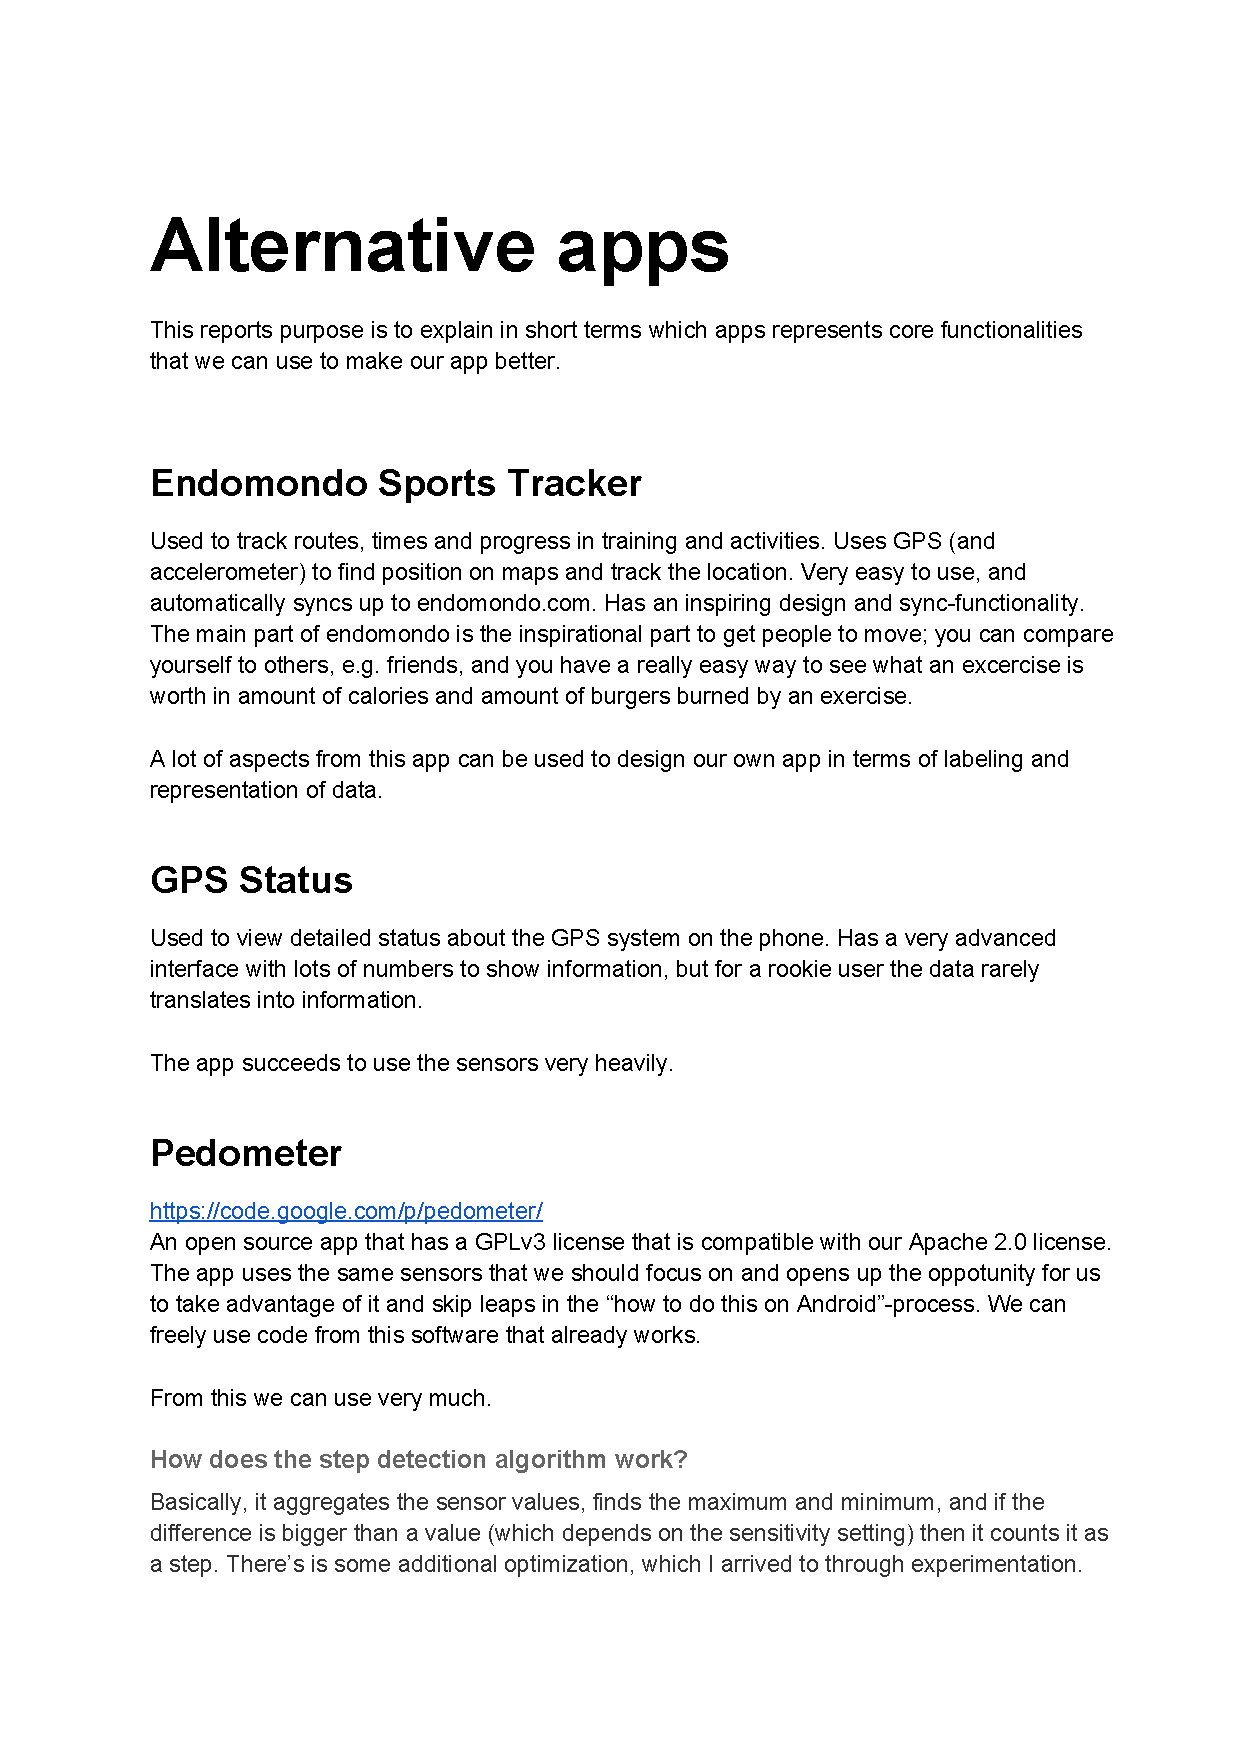
\includepdf[pages={-}]{Res/AlternativeAppsReport}

\section{Research Reports}
Fields that the team had little experience with was researched by one or two members, who wrote a summary for the rest of the team. The content of these reports was a part of the project, and therefor it was appropriate to include them. 

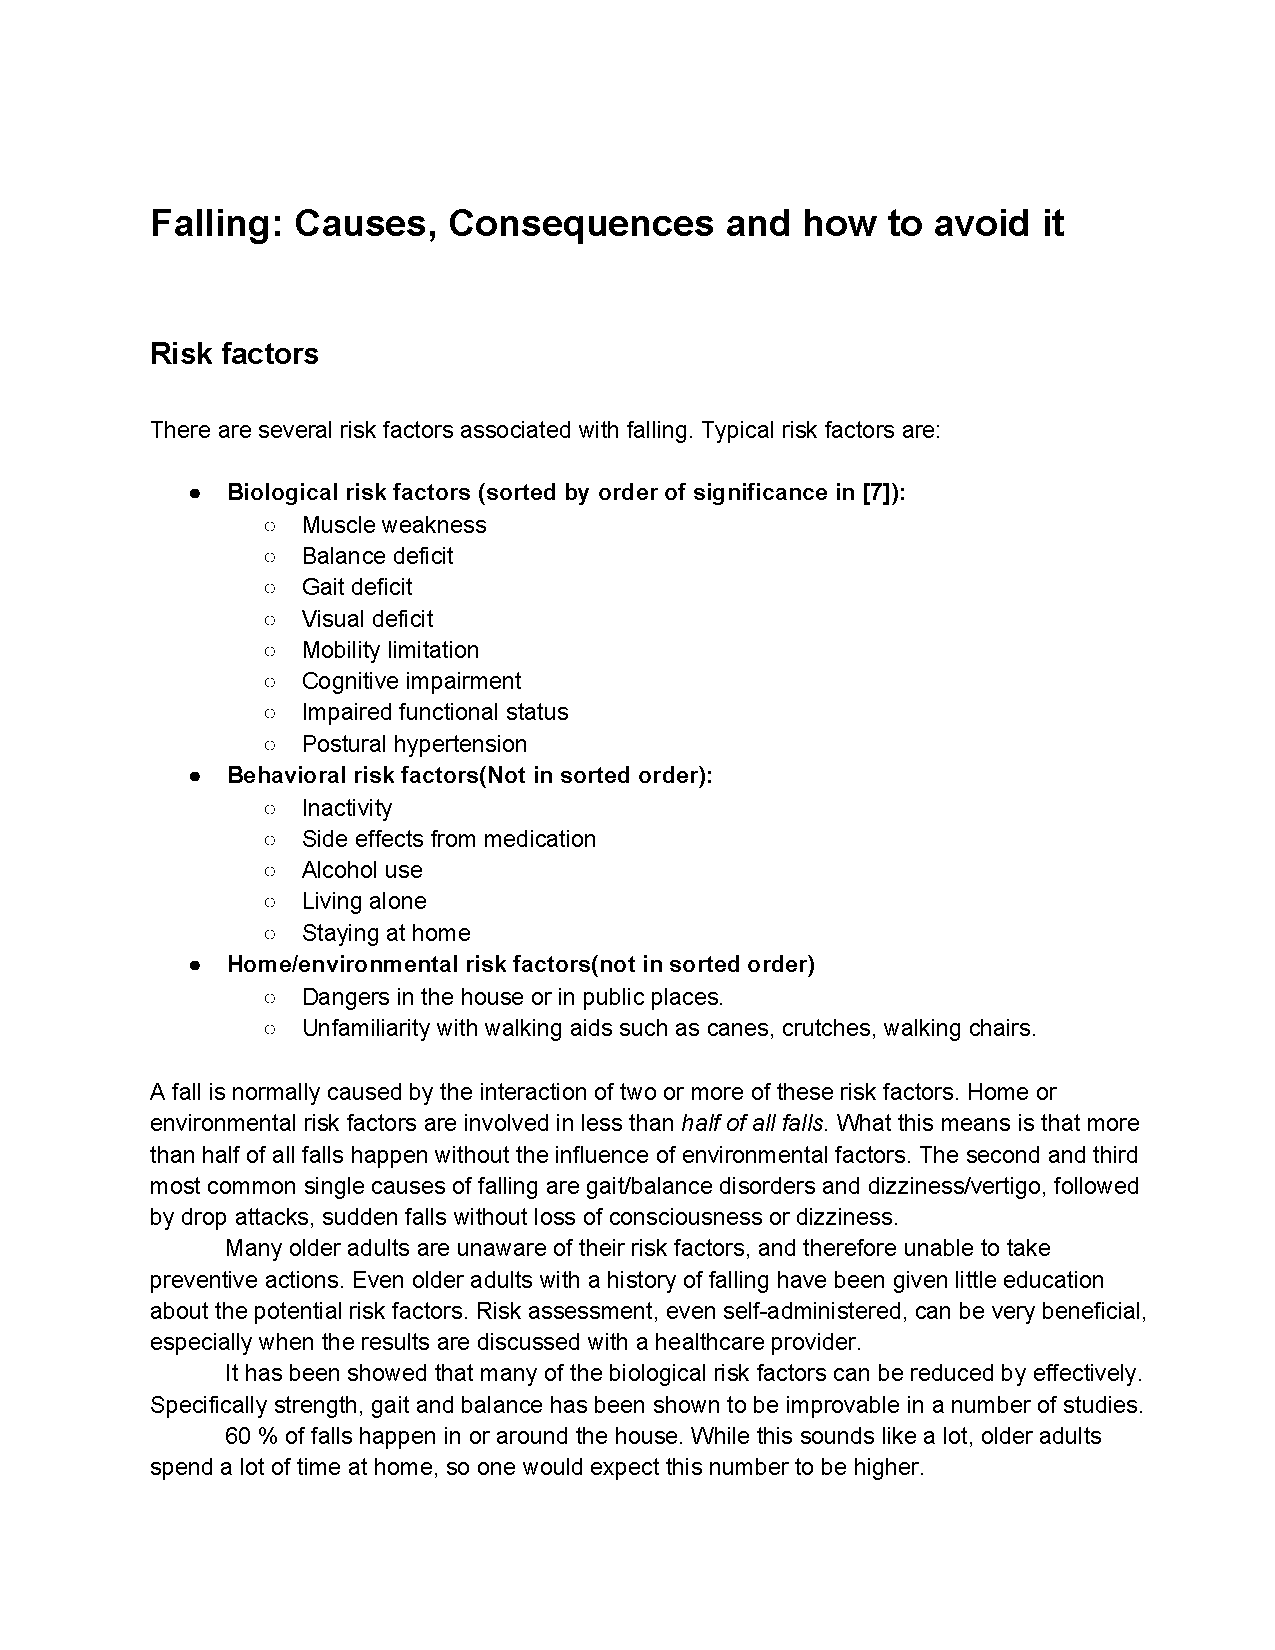
\includepdf[pages={-}]{Res/FallingCausesConsequences}


